% SC4024 --- Chapter 1: Visualisation Foundations & Perception (0->100 ground-up)
\chapter{Visualisation Foundations \& Perception}
\label{ch:foundations}
\sloppy

\begin{quote}
\emph{``A picture is worth a thousand numbers.''} --- But only if the picture is honest, legible, and matched to how eyes and brains actually work. This chapter asks what visualisation is and why perception sets its limits.
\end{quote}

\noindent\fbox{\parbox{\dimexpr\linewidth-2\fboxsep-2\fboxrule}{%
\textbf{From zero: we build here, no prior visualisation needed.} We assume only sets, numbers, and curiosity about pictures. Every notion---data table, visual channel, pre-attentive pop-out---is motivated by intuition, then defined, then exercised. No prior bachelor's knowledge is required.}}
\vspace{0.4em}

\section*{Learning Outcomes}
After this chapter you will be able to:
\begin{enumerate}[label=(L\arabic*)]
    \item define data visualisation and distinguish exploratory, explanatory, and presentational goals;
    \item explain the human visual pipeline from retina to cortex and pre-attentive processing;
    \item state Weber--Fechner and Stevens laws and predict perceived magnitude;
    \item rank visual channels by effectiveness for quantitative, ordinal, and nominal data;
    \item apply the Munzner nested model to characterise a visualisation design.
\end{enumerate}

% ============================================================
\section{What Is Data Visualisation?}
\label{sec:what-is-vis}
\paragraph{Intuition.} Anscombe's quartet is four datasets with identical means, variances, and correlations---yet their scatterplots look utterly different. Numbers hide structure that pictures reveal. Visualisation is the deliberate translation of data into a picture so that structure becomes visible without calculation.

\paragraph{Formal view.} A dataset is a collection of \emph{items} with \emph{attributes} (columns). A visualisation specifies a mapping $f: \text{data} \to \text{marks} \times \text{channels}$ rendered as an image, optionally interactive. Card, Mackinlay, and Shneiderman's reference model refines this into a pipeline: raw data $\to$ data tables $\to$ visual structures $\to$ views. Each stage transforms representation; each choice can help or mislead.

\begin{definition}[Visualisation pipeline]\label{def:pipeline}
\emph{Data transformation} cleans and derives data. \emph{Visual mapping} assigns data attributes to \emph{marks} (point, line, area, volume) and \emph{visual channels} (position, length, angle, colour, size, shape). \emph{View transformation} maps the visual structure to screen coordinates, handling zoom, pan, and clipping.
\end{definition}

\begin{figure}[h]\centering
\begin{tikzpicture}[scale=0.82,every node/.style={font=\scriptsize}]
\node[draw,thick,fill=blue!14,rounded corners=4pt,minimum width=2.2cm,minimum height=1.0cm,align=center] (raw) at (0,0) {Raw data\\{\tiny files, sensors}};
\node[draw,thick,fill=green!14,rounded corners=4pt,minimum width=2.2cm,minimum height=1.0cm,align=center] (tab) at (3.6,0) {Data tables\\{\tiny items $\times$ attributes}};
\node[draw,thick,fill=orange!15,rounded corners=4pt,minimum width=2.2cm,minimum height=1.0cm,align=center] (vis) at (7.2,0) {Visual structure\\{\tiny marks + channels}};
\node[draw,thick,fill=violet!12,rounded corners=4pt,minimum width=2.2cm,minimum height=1.0cm,align=center] (view) at (10.8,0) {View\\{\tiny rendered image}};
\draw[->,thick,>=Stealth] (raw) -- (tab) node[midway,above,font=\tiny] {transform};
\draw[->,thick,>=Stealth] (tab) -- (vis) node[midway,above,font=\tiny] {visual map};
\draw[->,thick,>=Stealth] (vis) -- (view) node[midway,above,font=\tiny] {view trans.};
\draw[->,thick,dashed,>=Stealth,blue!60!black] (view.south) -- ++(0,-0.7) -| (tab.south) node[pos=0.25,below,font=\tiny] {interaction loop};
\node[font=\tiny,fill=yellow!10,draw=gray!40,rounded corners=2pt,inner sep=3pt] at (5.4,-1.6) {\textcolor{blue!60!black}{$\blacksquare$ data} \quad \textcolor{green!50!black}{$\blacksquare$ tables} \quad \textcolor{orange!70!black}{$\blacksquare$ visual} \quad \textcolor{violet!60!black}{$\blacksquare$ view}};
\end{tikzpicture}
\caption{The Card--Mackinlay--Shneiderman visualisation pipeline. Interaction can feed back to any earlier stage; the forward path is data $\to$ picture.}
\label{fig:pipeline}
\end{figure}

Three goals orient design: \emph{explore} (find unknown patterns; analyst does not know what is there), \emph{explain} (communicate a known finding; audience must grasp it), and \emph{present} (enable repeated lookup; dashboards). The same data needs different pictures for different goals.

% ============================================================
\section{How Eyes See: The Visual System}
\label{sec:visual-system}
\paragraph{Intuition.} Look at a field of blue dots with one red dot. The red dot leaps out instantly---you do not scan dot by dot. That leap is \emph{pre-attentive} processing: before conscious attention, the visual cortex flags certain features in parallel across the whole field.

\paragraph{Formal view.} Light hits photoreceptors (rods and cones), retinal ganglion cells extract contrast, LGN relays to primary visual cortex V1 which detects edges and orientation, then higher areas separate form, colour, and motion. Pre-attentive features include hue, intensity, size, orientation, and motion. Conjunctions (e.g.\ red vertical among red horizontal and blue vertical) require serial search and are slow.

\begin{definition}[Weber--Fechner and Stevens]\label{def:perception-laws}
Weber's law: just-noticeable difference $\Delta I / I = k$ (constant). Fechner's law integrates this: perceived sensation $S = k \log I$. Stevens' power law refines it: $S = k I^{n}$ where $n$ depends on modality ($n\approx0.33$ for brightness, $\approx0.7$ for length, $\approx1$ for line length judged naively, $>1$ for electric shock).
\end{definition}

These laws matter: if perception is logarithmic, linear encodings of brightness will be misread; if length is underestimated, bar charts need careful baselines.

\begin{figure}[h]\centering
\begin{tikzpicture}[scale=0.78,every node/.style={font=\scriptsize}]
% pre-attentive demo: pop-out vs conjunction
\begin{scope}
\node[font=\footnotesize\bfseries] at (2.0,3.2) {Pop-out: hue};
\foreach \x in {0,...,4} \foreach \y in {0,...,3} {
  \pgfmathsetmacro{\dx}{0.75*\x + 0.15*rand}
  \pgfmathsetmacro{\dy}{0.65*\y + 0.15*rand}
  \fill[blue!55] (\dx,\dy) circle (0.14);
}
\fill[red!75] (1.5,1.3) circle (0.16);
\node[font=\tiny,fill=red!10,rounded corners=2pt] at (1.5,-0.5) {red target pops out};
\end{scope}
\begin{scope}[xshift=5.2cm]
\node[font=\footnotesize\bfseries] at (2.0,3.2) {Conjunction: hue+shape};
\foreach \x in {0,...,4} \foreach \y in {0,...,3} {
  \pgfmathparse{int(mod(\x+\y,2))}\let\p\pgfmathresult
  \ifnum\p=0 \fill[blue!55] (0.75*\x,0.65*\y) circle (0.14);
  \else \fill[blue!55] (0.75*\x,0.65*\y) rectangle +(0.26,0.26); \fi
}
\fill[red!75] (1.5,1.95) circle (0.14);
\fill[red!75] (2.25,0.65) rectangle +(0.26,0.26);
\node[font=\tiny,fill=orange!10,rounded corners=2pt] at (1.7,-0.5) {search is serial, slow};
\end{scope}
\begin{scope}[xshift=10.2cm]
\node[font=\footnotesize\bfseries] at (1.6,3.2) {Retina $\to$ cortex};
\draw[fill=orange!14,draw=orange!60!black,thick] (0,2.0) circle (0.35) node[font=\tiny] {retina};
\draw[->,thick,>=Stealth] (0.4,2.0) -- (1.1,2.0) node[midway,above,font=\tiny] {LGN};
\draw[fill=violet!14,draw=violet!60!black,thick,rounded corners=3pt] (1.1,1.4) rectangle (2.3,2.6) node[pos=.5,align=center,font=\tiny] {V1\\{\tiny edges}};
\draw[->,thick,>=Stealth] (2.3,2.0) -- (2.9,2.0);
\draw[fill=blue!12,draw=blue!60!black,thick,rounded corners=3pt] (2.9,1.5) rectangle (4.0,2.55) node[pos=.5,align=center,font=\tiny] {higher\\{\tiny form/col.}};
\fill[green!14] (0.2,0.4) rectangle (1.4,1.0); \node[font=\tiny] at (0.8,0.7) {pre-att.};
\fill[red!10] (1.6,0.4) rectangle (2.8,1.0); \node[font=\tiny] at (2.2,0.7) {attention};
\end{scope}
\node[font=\tiny,draw=gray!40,fill=yellow!8,rounded corners=2pt,inner sep=3pt] at (6.0,-1.15) {\textcolor{red!70!black}{$\blacksquare$ target} \quad \textcolor{blue!60!black}{$\blacksquare$ distractors} \quad \textcolor{orange!70!black}{$\blacksquare$ retina} \quad \textcolor{violet!60!black}{$\blacksquare$ cortex}};
\end{tikzpicture}
\caption{Pre-attentive processing: hue pops out in parallel (left); conjunctions of hue and shape require serial search (centre). Right: schematic visual pipeline.}
\label{fig:preattentive}
\end{figure}

% ============================================================
\section{Visual Channels and Effectiveness}
\label{sec:channels}
\paragraph{Intuition.} To show a number you can make a bar longer, a dot higher, a circle bigger, or a patch darker. Some of these are effortlessly precise (position), others are vague (colour saturation). Choosing the channel determines whether the reader gets the answer in a glance or a guess.

\begin{definition}[Marks and channels after Bertin/Mackinlay]\label{def:channels}
A \emph{mark} is a geometric primitive: point, line, area. A \emph{channel} controls a mark's appearance: position ($x,y$), length, angle, area, volume, colour hue/saturation/luminance, shape, texture, motion. Data attributes are typed as quantitative (ordered, arithmetic), ordinal (ordered, no arithmetic), or nominal (categorical). A channel's \emph{expressiveness} is whether it can encode the attribute type without implying false properties; its \emph{effectiveness} is perceptual accuracy.
\end{definition}

Mackinlay's ranking (validated by Cleveland--McGill) orders channels by quantitative judgment accuracy: position on common scale $>$ length $>$ angle/slope $>$ area $>$ volume $>$ colour. For nominal data, hue and position dominate; length misleadingly implies order and magnitude.

\begin{figure}[h]\centering
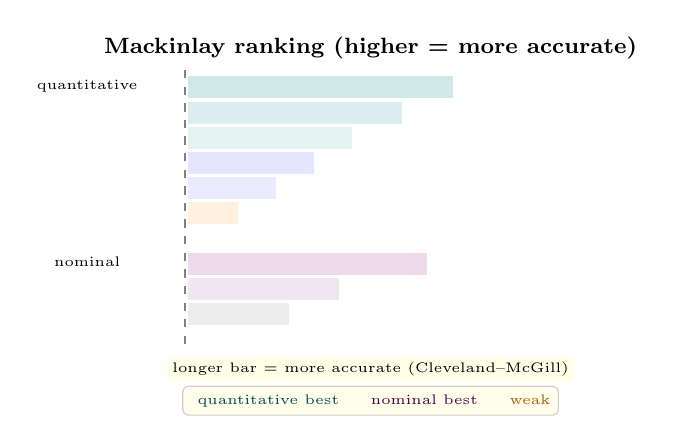
\begin{tikzpicture}[scale=0.80,every node/.style={font=\scriptsize}]
\node[font=\footnotesize\bfseries] at (4.5,5.6) {Mackinlay ranking (higher = more accurate)};
% quantitative bars
\node[font=\tiny,align=right] at (0,5.0) {quantitative};
\fill[teal!18] (1.6,4.8) rectangle (5.8,5.15) node[pos=.5,font=\tiny] {position};
\fill[teal!14] (1.6,4.4) rectangle (5.0,4.75) node[pos=.5,font=\tiny] {length};
\fill[teal!10] (1.6,4.0) rectangle (4.2,4.35) node[pos=.5,font=\tiny] {angle};
\fill[blue!10] (1.6,3.6) rectangle (3.6,3.95) node[pos=.5,font=\tiny] {area};
\fill[blue!8] (1.6,3.2) rectangle (3.0,3.55) node[pos=.5,font=\tiny] {volume};
\fill[orange!12] (1.6,2.8) rectangle (2.4,3.15) node[pos=.5,font=\tiny] {colour};
% nominal
\node[font=\tiny,align=right] at (0,2.2) {nominal};
\fill[violet!14] (1.6,2.0) rectangle (5.4,2.35) node[pos=.5,font=\tiny] {position/hue};
\fill[violet!10] (1.6,1.6) rectangle (4.0,1.95) node[pos=.5,font=\tiny] {shape};
\fill[gray!14] (1.6,1.2) rectangle (3.2,1.55) node[pos=.5,font=\tiny] {size (weak)};
\draw[thick,dashed,gray] (1.55,0.9) -- (1.55,5.3);
\node[font=\tiny,fill=yellow!10,rounded corners=2pt,inner sep=2pt] at (4.5,0.5) {longer bar = more accurate (Cleveland--McGill)};
\node[font=\tiny,draw=gray!40,fill=yellow!8,rounded corners=2pt,inner sep=3pt] at (4.5,-0.0) {\textcolor{teal!60!black}{$\blacksquare$ quantitative best} \quad \textcolor{violet!60!black}{$\blacksquare$ nominal best} \quad \textcolor{orange!70!black}{$\blacksquare$ weak}};
\end{tikzpicture}
\caption{Effectiveness ranking of channels. Position dominates for quantitative data; hue and position dominate for nominal. Colour luminance is poor for precise quantity.}
\label{fig:mackinlay}
\end{figure}

\begin{example}[Anscombe with four pictures]\label{ex:anscombe}
Four datasets share $\bar{x}=9$, $\bar{y}=7.5$, correlation $\approx0.82$, regression $y=3+0.5x$. Plotted, one is linear, one is curved, one has an outlier, one is a vertical line with one far point. A table of summary statistics cannot distinguish them; a scatterplot can. This motivates the entire course.
\end{example}

\begin{lstlisting}[language=Python, caption={Anscombe's quartet: same stats, four pictures.}, label={lst:anscombe}]
import matplotlib.pyplot as plt

# Anscombe quartet (first few rows shown; full 11 rows per set)
anscombe = {
  "I":  ([10,8,13,9,11,14,6,4,12,7,5],
         [8.04,6.95,7.58,8.81,8.33,9.96,7.24,4.26,10.84,4.82,5.68]),
  "II": ([10,8,13,9,11,14,6,4,12,7,5],
         [9.14,8.14,8.74,8.77,9.26,8.10,6.13,3.10,9.13,7.26,4.74]),
}
fig, axes = plt.subplots(1, 2, figsize=(8,3))
for ax, (k,(xs,ys)) in zip(axes, anscombe.items()):
    ax.scatter(xs, ys, c="steelblue", edgecolor="white")
    ax.set_title(k); ax.set_xlim(2,16); ax.set_ylim(2,12)
plt.tight_layout(); plt.savefig("anscombe.pdf")
\end{lstlisting}

\begin{lstlisting}[language=Python, caption={Pre-attentive intuition and Stevens law sketch.}, label={lst:stevens}]
import numpy as np, matplotlib.pyplot as plt

# Stevens power law: perceived = k * I^n
I = np.linspace(0.1, 10, 200)
for n, label in [(0.33,"brightness"), (0.7,"length"), (1.0,"line")]:
    plt.plot(I, I**n, label=f"n={n} {label}")
plt.xlabel("physical intensity I"); plt.ylabel("perceived S")
plt.legend(); plt.title("Stevens power law S=kI^n")
plt.savefig("stevens.pdf")
\end{lstlisting}

% ============================================================
\section{The Nested Model of Design}
\label{sec:nested}
\paragraph{Intuition.} A visualisation can fail at many levels: the wrong question, the wrong data abstraction, the wrong picture, or the wrong pixels. Tamara Munzner's nested model stacks these choices so a failure at an outer layer cannot be rescued by polishing an inner one.

Four nested levels: \emph{domain situation} (who are the users, what do they need?), \emph{data/task abstraction} (what data and tasks, precisely?), \emph{visual encoding/interaction} (what marks, channels, and interactions?), \emph{algorithm} (how to compute it fast and correctly?). Validation flows outward: algorithm benchmarks, encoding studies, abstraction interviews, domain field studies.

\begin{remark}[Why this book follows intuition$\to$formal$\to$example]\label{rem:nested-flow}
Each chapter mirrors the nested model: we start with the human and the question (domain), abstract the data, choose the picture, then show how to build it. Exercises ask you to move one layer outward and re-validate.
\end{remark}

% ============================================================
\section{Why Perception Constrains Design}
\label{sec:perception-design}
Even a correct pipeline fails if it asks eyes to do what they cannot. Two rules follow: never encode precise quantities in colour saturation alone, and never rely on angle or area when position would suffice. Interactive highlighting can rescue a weak channel by recruiting pre-attentive pop-out (e.g.\ hover turns a faint line red), but it cannot fix a fundamentally mismatched mapping. The next chapter turns these constraints into a systematic vocabulary.

% ============================================================
\section{Chapter Notes}
Visualisation as a field crystallised in the 1980s--90s (Bertin 1967 Semiology of Graphics; Card et al.\ 1999 Readings in Information Visualization). Mackinlay's APT (1986) automated channel choice; Cleveland and McGill (1984) measured channel accuracy; Munzner (2014) unified design as the nested model. Tufte (1983) and Ware (2020) connected design honesty to perception. The next chapter formalises data types and the channel vocabulary introduced here.

% ============================================================
\section{Exercises}
\label{sec:ch01-exercises}
\begin{enumerate}[label=E1.\arabic*, leftmargin=*, itemsep=0.8em]
    \item \textbf{Anscombe extended.} Compute $\bar{x},\bar{y},$ variance, and Pearson $r$ for Anscombe set III by hand for 5 points and verify equality across sets. Plot all four sets and describe in one sentence how each would mislead a model fitted only to summaries.
    \item \textbf{Stevens fitting.} Given perceived brightness judgments $S=[2,3.6,5.8]$ at intensities $I=[1,4,9]$, fit $S=kI^{n}$ in log-log space (linear regression of $\log S$ on $\log I$). Report $n$ and interpret whether brightness is compressive ($n<1$).
    \item \textbf{Channel ranking task.} For the task ``compare GDP of 6 countries to within 10\% accuracy'' propose three encodings (position, area, colour luminance) and rank them using Mackinlay/Cleveland--McGill. Justify with a sketch and one-sentence effectiveness argument per channel.
    \item \textbf{Nested-model mapping.} Take the visualisation ``COVID-19 dashboard with map + time series + hospital bar chart.'' Assign each component to a nested-model level, state one threat to validity per level, and propose one validation method per threat.
    \item \textbf{Misleading chart critique.} Find a chart with a truncated y-axis (or 3-D extrusion) online; redesign it with a zero baseline (or 2-D bars) and explain the perceptual error the original induces using Weber--Fechner or Stevens reasoning.
\end{enumerate}
% End of Chapter 1
